\if0
先述のHL7などの共通の規格が活用されていない現実があるので,
いろんな規格の差を吸収できるようなアプリは需要があると考える.
三重県にこのような医療ネットワークを実現するためのたたき台として
本研究では開発を進めた.
\fi



\subsection{SQL版の概要}
  特定の病気にかかっている複数人の患者の医療情報が記載された
  エクセルファイルを医療関係者から提供していただいた.
  医療情報として検査値,投薬についての情報などが記載されていた.
 このエクセルのデータのみを受け付けるWebアプリケーション
  をDjangoで開発した.

  検査値,投薬についての情報を患者の認可のもとで収集し,
  SQLデータベースに保存する.
  患者に認可をされた医療関係者は情報の参照,書き込みが可能となる.

  このサービスを実現するために後述する機能を実装した.

  本研究ではユーザとして患者と医療関係者の2つの立場があることを
  想定している.
  ユーザモデルは二者を区別できるように実装し,
  二者で異なる使い方ができるようにした.



\subsection{SQL版が有する機能}
  \subsubsection{データ入力}
    データベースには提供していただいたエクセルファイルの記述方法に対応する
    SQLのテーブルを用意している.
    ファイルをアプリケーションが図\ref{DjangoFileio}の
    ページで受け取ると検査値と投薬についての
    情報を医療情報をデータベースへ入力することができる.

  \subsubsection{データ閲覧}
    診断データは表にして、縦方向に診断項目,
    横方向に診断を行った日をとっている.
    空白部分はデータが入力されていない項目である.
    (図\ref{DjangoTable})


    投薬データはある薬をどれだけの期間服用しているかを
    わかりやすくするためにガントチャートのように表示している.
    色によってカテゴリの視認性を向上させたため,
    同時に服用することが好ましくない薬の組み合わせや
    過度な投薬を発見しやすい.(図\ref{DjangoGantt})

  \subsubsection{権限の付与}
    患者の医療情報をどの医療関係者が操作することができるかを
    患者自身が選択する.
    認可には段階を設けた.
    具体的には,閲覧不可,閲覧可能と書き込み可能の
    3段階の認可を用意することである.
    これにより,医療関係者は患者の意志を尊重しながら
    医療情報を活用することができる.

\subsection{医療関係者の利用方法}
  患者によって閲覧,書き込みが許可された医療関係者は,
  他の医療関係者によって入力された医療情報を
  Webインターフェース上で閲覧することができる.
  また,検査,診断などによって得られた
  新たな医療情報を追記することができる.

\subsection{患者の利用方法}
  患者はWebインターフェースにより自身の医療情報の
  閲覧をすることができるので,図\ref{DjangoGantt}の
  ガントチャートによって処方すべき治療薬の種類,期間,数量を
  確認することができる.

  さらに,医療情報共有システムを導入していない医療機関に
  かかるときは患者の端末で自身の医療情報を表示することで
  医療関係者に既往歴を閲覧させることができる.


    \begin{figure}[htbp]
        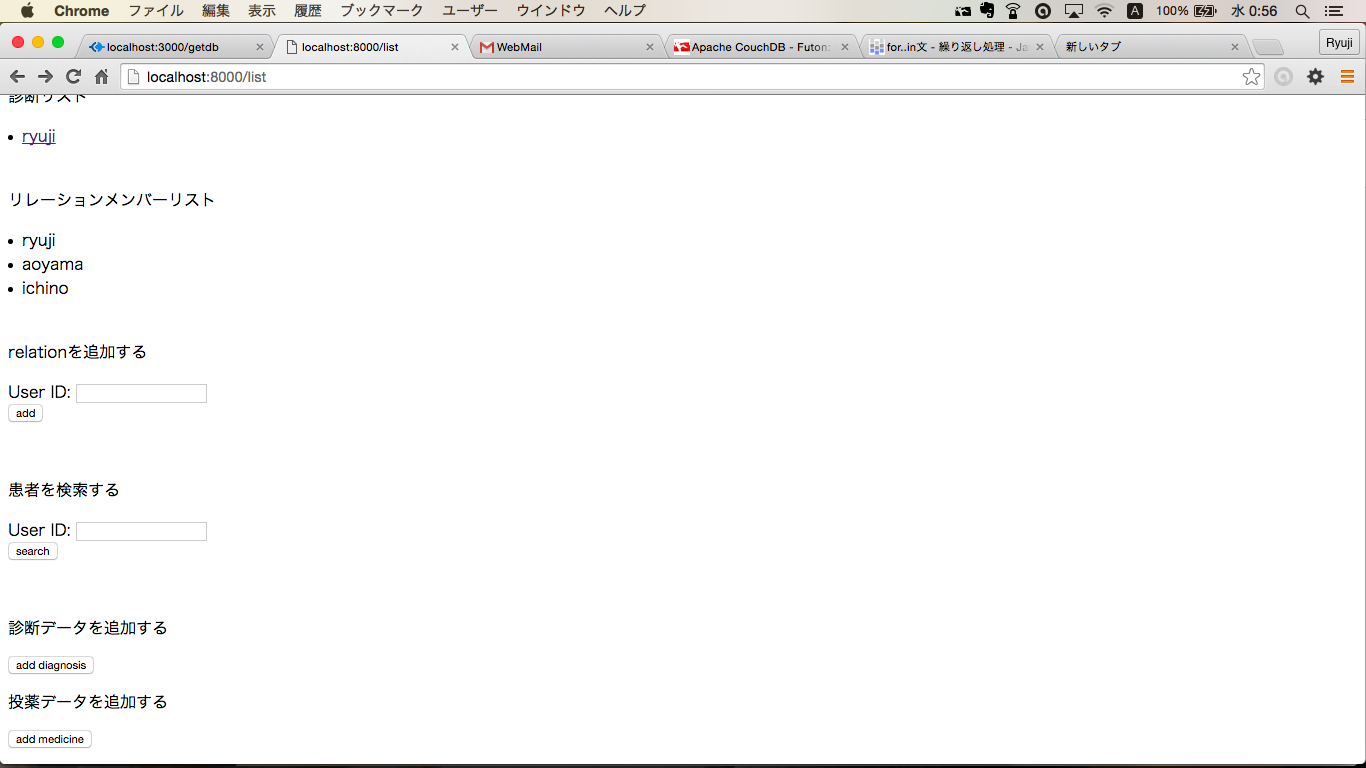
\includegraphics[width=5cm, bb=0 0 437 688]{./gazou/DjangoFileio.png}
      \caption{データ入力画面}
      \label{DjangoFileio}
    \end{figure}

    \begin{figure}[htbp]
        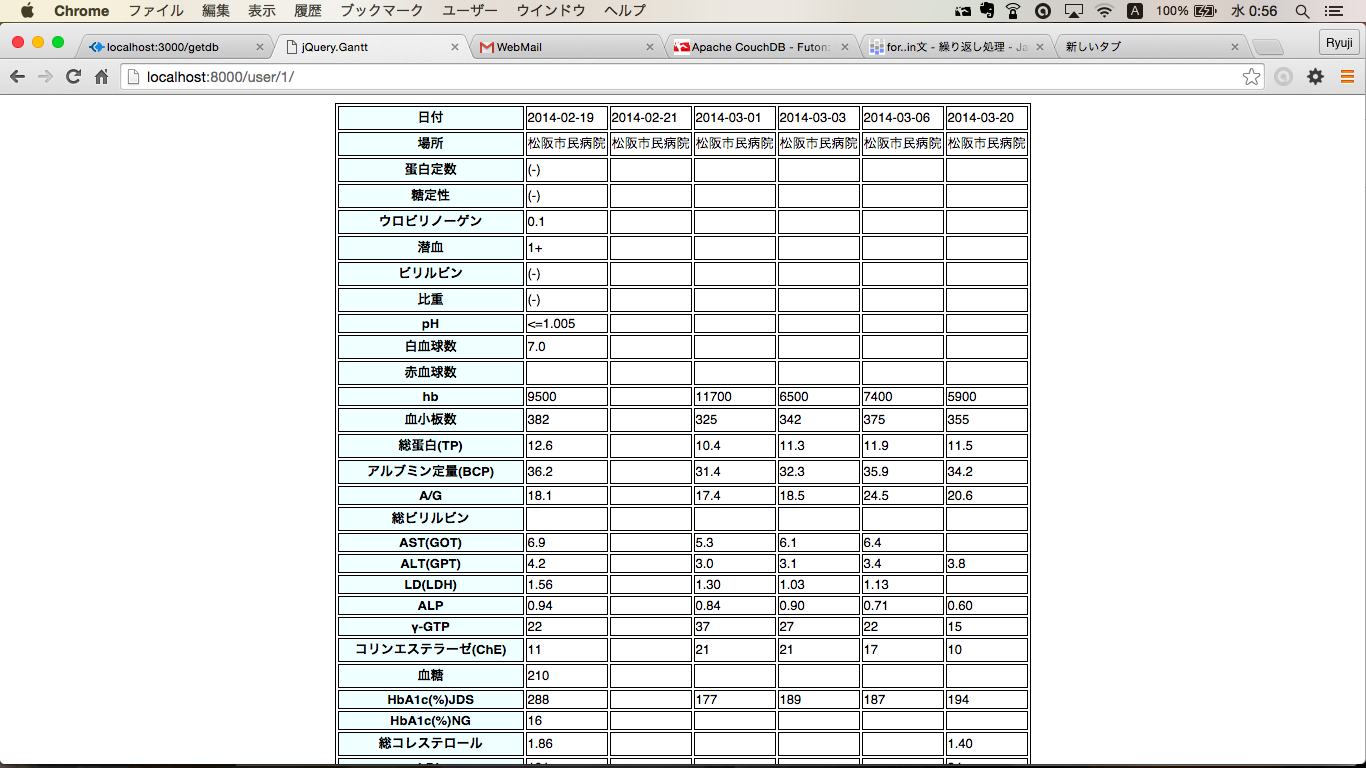
\includegraphics[width=5cm, bb=0 0 437 688]{./gazou/DjangoTable.png}
      \caption{表によるデータ閲覧}
      \label{DjangoTable}
    \end{figure}

    \begin{figure}[htbp]
        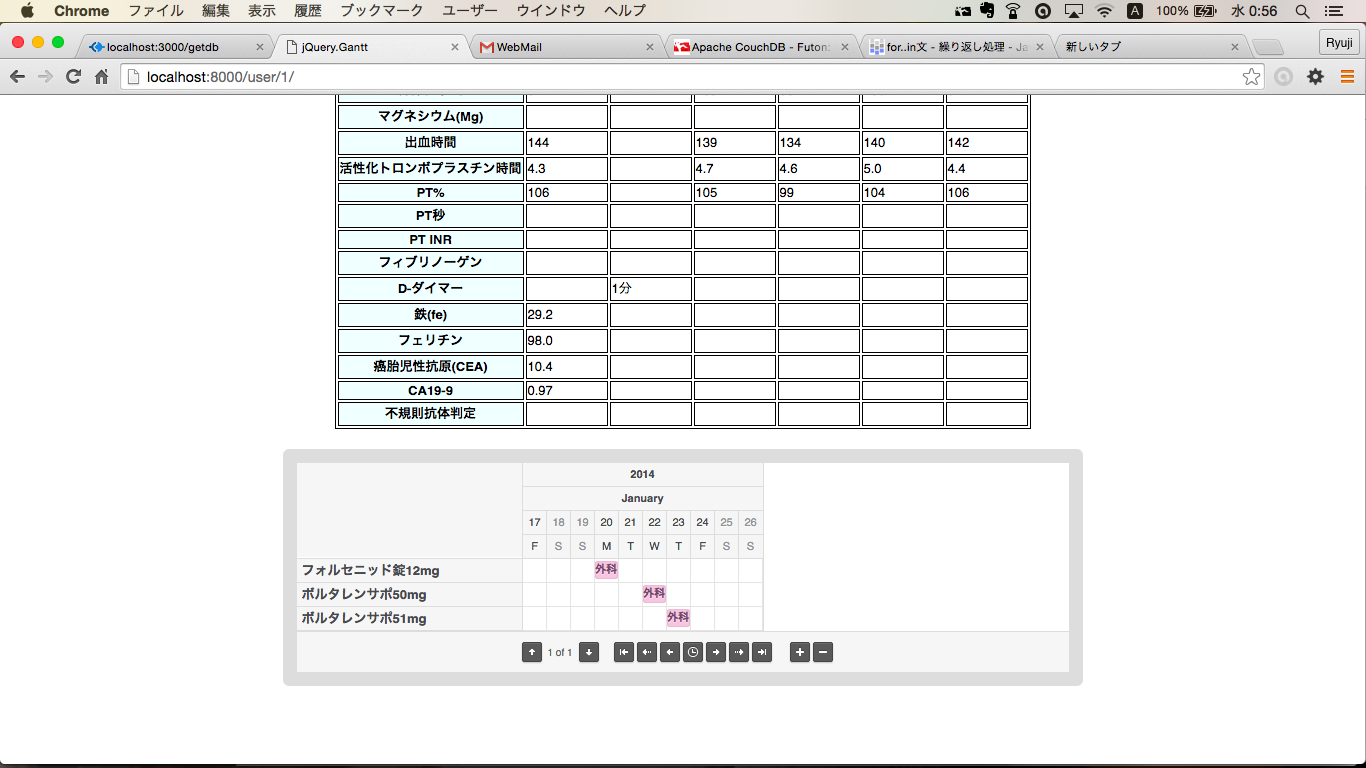
\includegraphics[width=5cm, bb=0 0 437 688]{./gazou/DjangoGantt.png}
      \caption{ガントチャートによるデータ閲覧}
      \label{DjangoGantt}
    \end{figure}


\if0
\subsection{SQL版の課題とフィードバック}

  開発アプリのデモンストレーションをデータを提供していただいた
  医療関係者に対して行った.
  そのときにいただいたWebアプリケーション改善のための意見の中で
  研究課題として任意の検査項目の抽出が挙げられる.

  他の意見はインターフェース寄りの要望が多かった.
  例えば,表によるデータの表示に対するフィードバックとして,
  任意の検査項目にハイライトをつけてほしいといった内容であったが,
  本研究で工数を割くことができなかったため開発を見送った.
\fi

\subsection{NoSQL版の目標設定}
  ひとつのフォーマットのみならず,
  これらのファイルでの入力を入力を受け付ける
  WebアプリケーションをCouchDBを用いて実装する.

  医療の現場からは電子カルテや血圧計の出力ファイルとして
  様々なCSVファイルが出力される.
  また,電子カルテに関してはHL7で規格化されたファイルが
  出力できることもある.

  異なるフォーマットの入力データから,同じ意味の項目であっても,
  厳密に同じ言葉を項目名にとっていないことがある.
  ここでは便宜的に異なる項目名であるが同じ意味の項目の群を
  同義キーと呼ぶ.

  この同義キーを関連付ける機能を実装する.
  これにより,同義キーのうちのひとつが検索される際に,
  その同義キーの群の項目も検索結果として反映させる.

  \if0
  ドキュメントの数だけSQLデータベースのテーブルを用意する必要がある.
  データを検索する際にはjoinしてから.
  比べてNoSQLならガンガン入れて,
  データを出すときにだけKeyの関連づけをすればよい.
  NoSQLならSQLに比べてテーブルを用意する分の
  コストがはぶけてる(と言えるかな).
  \fi
